\documentclass{article}
\usepackage{tikz, comment}
\usepackage{pifont}
\usepackage{fontspec}
\usetikzlibrary{arrows, decorations.markings, decorations.pathreplacing}
\begin{comment}
:Title: Not defined yet
:Tags: area using polar coordinates, polar integral formula ;moment;polar coordinates;sine, sin ;eccentricity of a conic section
:Prob: 0.4257;0.4097;0.4024;0.4008;0.3858
:Slug: No name yet

Description Here.........
\end{comment}
\begin{document}\centering

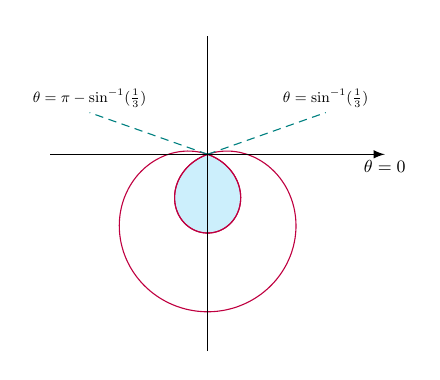
\begin{tikzpicture}[>=latex,xscale=.5*1, yscale=.5*1][font=\sf\small]

%\draw[xstep=1cm,ystep=1cm,color=gray!80] (0, -1) grid (8, 8);

\draw[purple, fill=cyan!20, samples=100, smooth, domain= 0.339837:pi-0.339837, variable=\t]
plot ({(1-3*sin(\t r))*cos(\t r)}, {(1-3*sin(\t r))*sin(\t r)});

\draw[purple, samples=100, smooth, domain=0:2*pi, variable=\t]
plot ({(1-3*sin(\t r))*cos(\t r)}, {(1-3*sin(\t r))*sin(\t r)});

\draw[densely dashed, teal, samples=100, smooth, domain=0:3, variable=\x]
plot ({\x}, {tan(0.339837 r)*(\x)})node[above, black, scale=0.6] {$\theta=\sin^{-1}(\frac{1}{3})$};

\draw[densely dashed, teal, samples=100, smooth, domain=0:-3, variable=\x]
plot ({\x}, {tan((pi-0.339837) r)*(\x)})node[above, black, scale=0.6] {$\theta=\pi - \sin^{-1}(\frac{1}{3})$};

\foreach \x in {}
\draw (\x,2pt/6) -- (\x,-2pt/6)
node[anchor=north] {\tiny$\x$}
;

\foreach \x in {}
\draw (\x,2pt/2.5) -- (\x,-2pt/2.5)
node[anchor=south] {\tiny$\x$}
;
\foreach \y in {}
\draw (-2pt/6,\y) -- (2pt/6,\y)
node[anchor=east] {\tiny $\y$}
;

\draw[->] (-4, 0) -- (4.5, 0)node[below, scale=0.7] {$\theta=0$} ;
\draw[] (0, -5) -- (0, 3)node[left] {};

%\node[yshift=0] at (-0.2/1, -0.2/1) {\tiny$0$};

\end{tikzpicture}
\end{document}